
\section{Setup \& Hardware}
All of our code was written from scratch.\newline\newline
The goal of our project was to create a working GA* implementation on GPU. To this end, we used C++ for serial implementations and CUDA programming to develop our GPU code. We evaluated our code on the GHC machines.\newline\newline

\section{Work Distribution}
The parallelism of our work comes from how we explore the frontier of the A* search more efficiently. The original A* algorithm as designed for sequential execution is not amenable to parallel speedup, so we used the GA* algorithm instead to judge parallel execution. \newline\newline
Each of our threads corresponded to one priority queue. It was responsible for popping the top node in the priority queue, and evaluating it for if it is the goal state and for finding its neighbors. With this approach, we could have \textit{thousands} of priority queues, which is especially useful in problems where the number of states increases exponentially, such as the slider problem we describe in the Results. In the rest of our algorithm, we encounter a lot of communication and synchronization. \newline\newline
We allocate a global array \verb|S| for storing all the neighbors that are being added to the frontier due to the expansion of the priority queue nodes. This array is accessible to all the threads. Once each thread generates the neighbors it expands in the current iteration, it adds those neighbors to \verb|S|.\newline\newline
We also allocate the hash table as a global variable. Once the threads populate the array \verb|S|, each thread works on deduplicating nodes in the array \verb|S| (not necessarily the nodes it added to \verb|S|!). This is done by looking at the global hash map for the same node and replacing it if there's a node in \verb|S| that has lower cost. If not, we discard this node from \verb|S|. \newline\newline
Finally, we redistribute the remaining nodes evenly to the many different priority queues. We do this by rearranging the indices in \verb|S| that correspond to the thread.

\begin{figure}
    \centering
    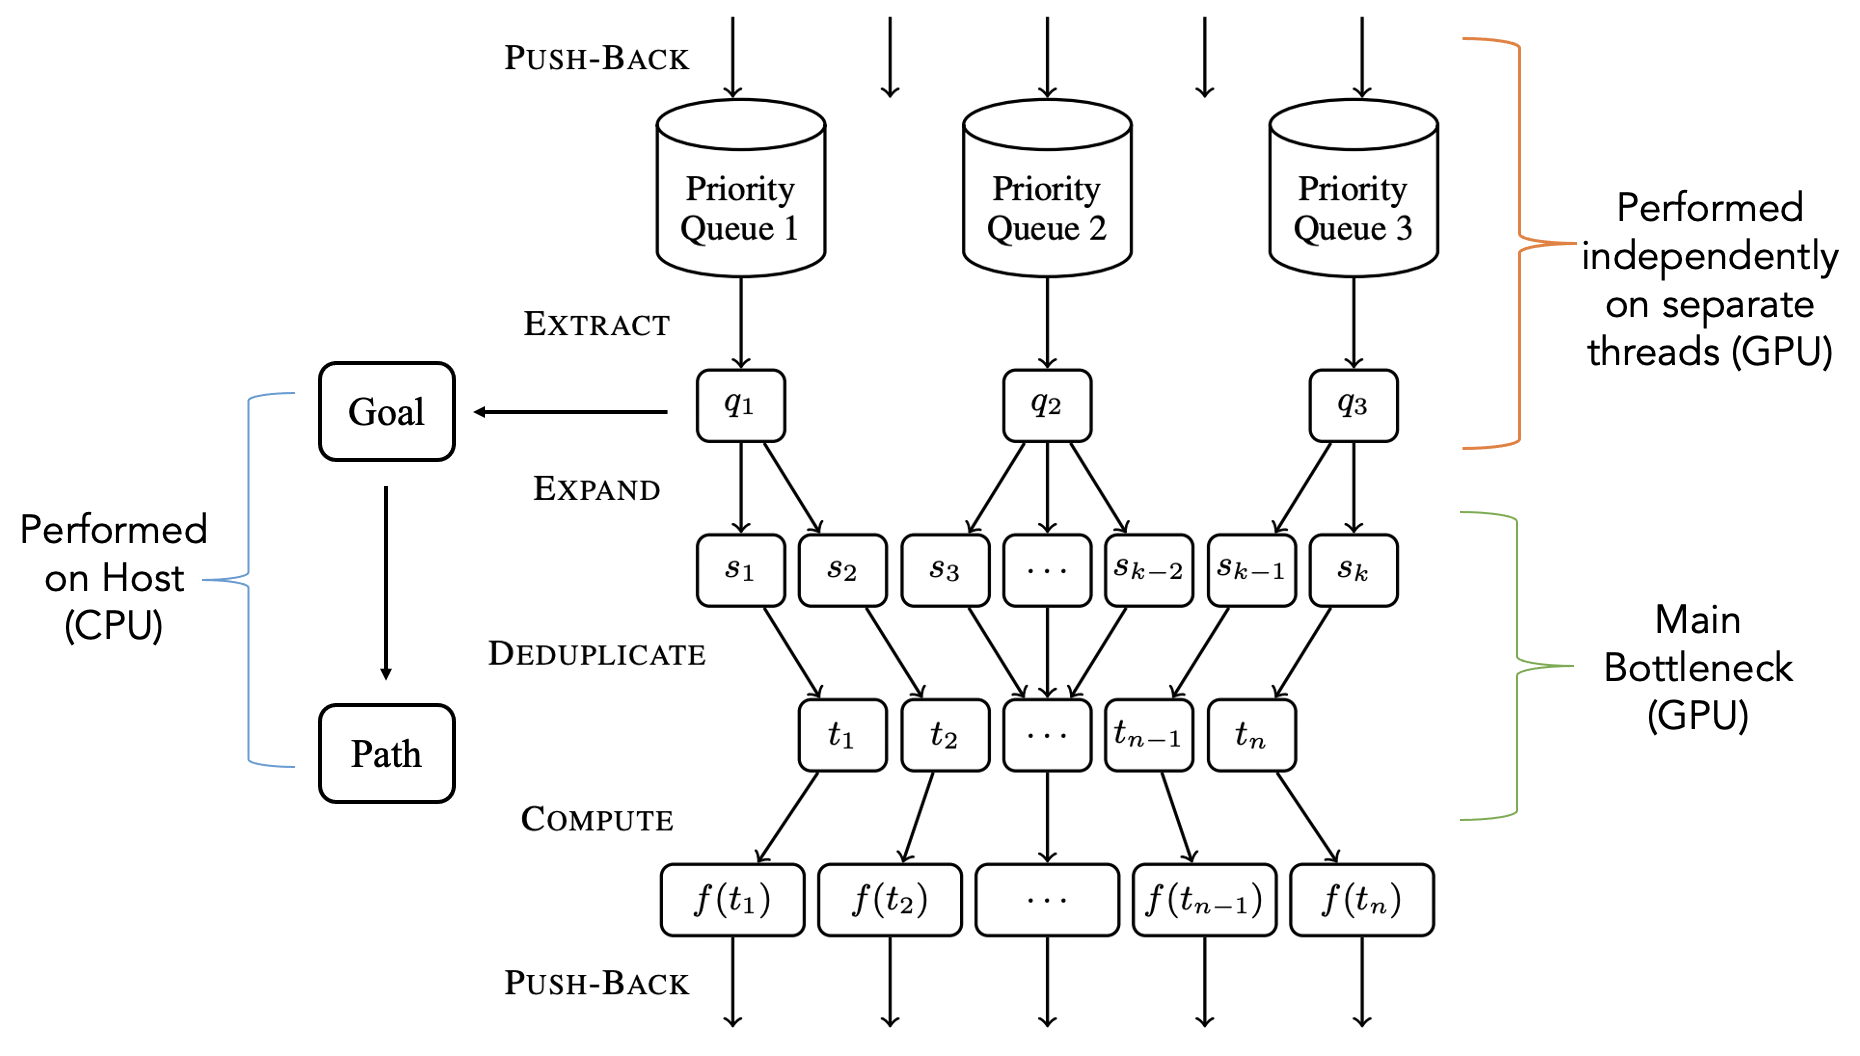
\includegraphics[scale=0.5]{figures/gastar_device.png}
    \caption{GA* workflow with relevant data structures (based on \cite{paper})}
    \label{fig:gastar_device}
\end{figure}

\section{Iterations of our Approach}
We began by implementing and verifying a sequential version of the original A* algorithm. These results are presented in the Results below. We then created a sequential version of the GA* algorithm that worked (i.e. it could run on a single CPU thread, not on CUDA. Nodes were mapped to a random priority queue so the structure imitated the final result we were hoping for). Finally, we made numerous attempts at a CUDA implementation for the GA* algorithm, but we were ultimately unsuccessful.\newline\newline
Along the way, we made a couple optimizations to our approach. We decided to allocate nodes in our frontier in \verb|S| in one ordering, and then \textbf{we redistribute the nodes to threads in a different order}. This way, by having nodes in different parts of the graph, the work done by the threads is evenly spread out. That is, we are less likely to run into situations where many priority queues are empty and do not have nodes to expand or add to \verb|S|.\newline\newline
Another idea we found was that we could optimize our deduplication to haves less synchronization and therefore potentially save time. There were two methods that \cite{paper} suggested for a parallel implementation of a hash table. The first one, Cuckoo Hashing, is a more complicated method that involved greater synchronization between threads. We opted to go with the second approach, Hashing with replacement, which required no synchronization at the cost of missing some duplicate nodes. We decided this tradeoff was acceptable because this approach would not affect the final path returned.